% IACR Transactions CLASS DOCUMENTATION
% Written by Gaetan Leurent gaetan.leurent@inria.fr (2016-2018)
%
% To the extent possible under law, the author(s) have dedicated all
% copyright and related and neighboring rights to this software to the
% public domain worldwide. This software is distributed without any
% warranty.
%
% You should have received a copy of the CC0 Public Domain Dedication
% along with this software. If not, see
% <http://creativecommons.org/publicdomain/zero/1.0/>.

\documentclass{iacrtrans}
\usepackage[utf8]{inputenc}
\usepackage[ruled,vlined,linesnumbered]{algorithm2e}
\usepackage[english]{babel}
\usepackage{subfig}

\usepackage{graphicx}
\usepackage{multicol}
\usepackage[nottoc]{tocbibind}




\graphicspath{ {figure/} }


\title[\texttt{iacrtans} class documentation]{\publname}
\subtitle{\LaTeX{} Class Documentation (v. 0.92)}

\begin{document}


\maketitle

% use optional argument because the \LaTeX command breaks the PDF keywords
\keywords[\publname, ToSC, TCHES, LaTeX]{\publname{} \and ToSC
  \and TCHES \and \LaTeX}

\begin{abstract}
  This document is a quick introduction to the \LaTeX{} class for the
  \publname{}.
\end{abstract}

\tableofcontents{}

\section{Silent zero store}
A silent store attempts to write a value matching the one already stored at the memory location. Silent stores occur frequently and up to $50\%$ of them can be eliminated with low implementation costs \cite{lepak2000silent}\cite{bell2000characterization}. Elimination of silent stores can result in $11\%$ performance speed up \cite{lepak2000silent}. Recent blog posts have shown that Intel has implemented silent stores into Skylake and Ice Lake microarchitectures \cite{downs_2020_ice} \cite{downs_2020_hardware}. However, instead of implementing general silent stores, Intel implements silent zero stores. Indeed, implementing general silent stores will result in more performance speed up, but it is also harder to detect than an all zero case and zeros overwriting zeros is one of the most common redundant writing scenarios. 

To be specific, for a silent zero store, a cacheline is marked as $isZero$ if it is all zero when allocated. By the time it is evicted from the cache, if the $isZero$ flag is still on, the writeback will be dropped regardless of whether the dirty flag is on. Even though the cacheline might have been modified after allocation, so long as it is all zero when evicted, the eviction will be treated as a clean eviction. Throughout this paper, we consider only the silent zero store case. We investigate possible security pitfalls in cryptography protocols caused by the silent zero store. In a multi-level caches, we assume there is a performance counter $perf_{zero}$ counting the number of redundant zeros overwriting zeros cases. 

\section{Attack model}
In our attack scenario, we assume a passive attacker that co-locates with the victim on the same machine. We assume the attacker is aware of the crypto protocol running on the machine and is able to access the $perf_{zero}$ before and after the execution of a function of his interests. However, the attacker cannot access $perf_{zero}$ any time of his choice, neither can he perform $FLush+Reload$ attacks to influence the cache access and eviction pattern. 

\section{Cryptography protocols}
\subsection{RSA}
RSA is a public-key cryptosystem. We will describe how to retrieve RSA static private key by introducing silent zero stores into RSA decryption. RSA decryption is a modular exponentiation: $m \equiv c^d$ mod $N$, where $c$ is the ciphertext being decrypted, $d$ the private key exponent, $N=pq$ the RSA modulus ($p$ and $q$ are two big prime numbers). The basis of RSA is the difficulty of factoring the modulus $N$. To keep the private key $d$ secret, the factors $p$ and $q$ should also be kept secret. Most implementations use the Chinese Remainder Theorem(CRT) to perform the exponentiation $c^d$. First, $d_p$ and $d_q$ are precomputed as: $d_p \equiv \frac{1}{e}$ mod $p-1$, $d_q \equiv \frac{1}{e}$ mod $q-1$, where $e$ is part of the public key ($de \equiv 1$ mod $\phi(pq) = (p-1)(q-1)$). Second, $m_p$ and $m_q$ are derived from $c$: $m_p \equiv c^{d_p}$ mod $p$, $m_q \equiv c^{d_q}$ mod $q$. Third, $m_p$ and $m_q$ are combined to derive $m$. 

There are different algorithms to compute $c^{d_p}$ mod $p$ and $c^{d_q}$ mod $q$. However, a common first step is to reduce $c$ with respect to $p$ and $q$: $c_p \equiv c$ mod $p$, $c_q \equiv c$ mod $q$. Assuming the ciphertext $c$ is in the form of a leading $1$ followed by a sequence of $0$. After the modular reduction $c_p \equiv c$ mod $p$, if $c<=p$, $c_p$ should remain as $c$, if $c>p$, $c_p$ would become $c-kp$ for some unknown $k$. Since the value of $k$ is unpredictable, it is highly unlikely that $c-kp$ will preserve the same form as $c$. Assuming the buffer representing $c_p$ initially is allocated with $0$, if $c<=p$, it will be overwritten with $0$ except the leading bit; if $c>p$ it will be overwritten by random data. Therefore, if the cacheline containing the buffer $c_p$ get evicted after modification, and the size of $c_p$ is bigger than that of a cacheline, silent zero stores will be generated only if $c<=p$. The ability to capture such silent zero stores will enable the attacker to decrypt the top \emph{(sizeofp-sizeofcacheline)} bits of $p$ in a binary search way as described in Algorithm \ref{tab:algRSA}. If $\emph{sizeofp} > \emph{2*sizeofcacheline}$, the attacker can completely factor $N$ and then retrieve the private key $d$ by using lattice-reduction techniques pioneered by Coppersmith \cite{coppersmith1997small}. 
\begin{algorithm}[H]
\SetAlgoLined
\textbf{Input: } ciphertext $c$ (size of $c$ equals to the size of $p$) \\
\textbf{Output: } Top \emph{(sizeofp-sizeofcacheline)} bits of $p$ \\
 \emph{bitsRecovered} = 1\;
 c = 10...0; \;
 \While{ bitsRecovered < (sizeofp-sizeofcacheline)}{
  $c_p \equiv c$ mod $p$ \;
  \eIf{Silent zero stores observed}{
   $c<=p$\;
   The \emph{bitsRecovered-th} bit of $p$ $=$ The \emph{bitsRecovered-th} bit of $c$\;
   Turn the \emph{(bitsRecovered+1)-th} bit of $c$ to 1\;
   }{
   $c>p$\;
   Turn the \emph{(bitsRecovered)-th} bit of $c$ to 0\;
  }
  \emph{bitsRecovered}++\;
 }
 \caption{Recover the RSA secret prime numbers}
 \label{tab:algRSA}
\end{algorithm}


\subsection{ECDH}
Elliptic-curve Diffie–Hellman (ECDH) is a key agreement protocol which allows two parties $A$ and $B$ to agree on a shared secret. We will describe how to retrieve ECDH static private key by introducing silent zero stores into the computation of the shared secret. An elliptic curve $E$ of order $n$ over a finite field $\mathbb{K}$ can be defined by its \emph{Weierstrass} equation: $y^2 = x^3+ax+b$. Given the primitive element $P$ on $E$, the party $A$ will choose an integer between $0$ and $n$ as the secret key $s_a$, and computes the scalar multiplication of $P$: $[s_a]P$ as her public key $p_a$. The party $B$ will choose an integer between $0$ and $n$ as the secret key $s_b$, and computes $[s_b]P$ as his public key $p_b$. $p_a$ and $p_b$ will be sent to the other party and the shared secret $s$ will be derived as: $[s_b][s_a]P$. The security of ECDH relies on the elliptic curve discrete logarithm problem (ECDLP): given $E$, $P$, $p_a$, it is assumed to be hard to recover the integer $s_a$ that satisfies $p_a=[s_a]P$. However, with silent zero stores, a malicious $B$ that co-locate with the victim $A$ can send out public key $p_b$ by his choice, and then retrieve the static private key $s_a$ by monitoring the occurrence of silent zero stores. There are different constant time algorithms that perform the scalar multiplication of points on elliptic curve. We discuss the two most popular ones: The Montgomery ladder algorithm and the fixed window algorithm. We assume the finite field $\mathbb{K}$ is at least as big as $2^{cachelineSize}$. We define the point $Z$ as the point with $x$ coordinate equals to $0$.

\subsubsection{Fixed window}
Algorithm \ref{tab:algFW} is the constant time fixed window algorithm for elliptic curve point multiplication. An attacker with the knowledge of the static secret key $s_a$ up to bit $i-1$, can calculate the relationship between $Q$ and the input point $p_b$: $Q_{i-1} = [scalar_{i-1}]p_b$. For iteration $i$, the attacker can brute force $s_{a_i}$ by sending $[((scalar_{i-1})*2^w + d_i)^{-1}]Z$ where $d_i$ ranges from $1$ to $2^w-1$. If a correct guess is made: $d_i = s_{a_i}$, the point $Q$ at the beginning of iteration $i+1$ will be the point $Z$. The multiplication $[2^w]Z$ will generate multiple zeros overwriting zeros. If the cacheline containing the zeros get evicted after modification, the $perf_{zero}$ will be incremented, which can be used as a side channel by the attacker to confirm the correctness of his guess. The window size $w$ used in this algorithm is usually around 5, so brute force the secret key $s_a$ window by window will not be computationally impossible. 

\begin{algorithm}[H]
\SetAlgoLined
\textbf{Input: } $p_b$, window size $w$, $s_a = s_{a_0} + 2^ws_{a_1} + 2^{2w}s_{a_2} + ... + 2^{mw}s_{a_m}$ \\
\textbf{Output: } $s = [s_a]p_b$ \\
 Precompute $[d]p_b$ for $d = 1...(2^w-1)$\;
 $Q = \emph{O}$\;
 \For{ $i = m$ down to $0$} {
     $Q = [2^w]Q$\;
     $Q = Q + [s_{a_i}]p_b$ using the precomputed table\;
  }
 \caption{Fixed window}
 \label{tab:algFW}
\end{algorithm}

\subsubsection{Montgomery Ladder}
Algorithm \ref{tab:algML} is the constant time left-to-right Montgomery ladder algorithm for elliptic curve point multiplication \cite{montgomery1987speeding}. An attacker with the knowledge of the static secret key $s_a$ up to bit $i-1$, can calculate the relationship between $R$, $S$ and the input point $p_b$ ($R_{i-1}=[scalar_{i-1}]p_b$, $S_{i-1}=[scalar_{i-1}']p_b$) before the iteration $i$. During iteration $i$, the points $R$ and $S$ will be swapped depending on $s_{a_i} \oplus \emph{swap}$. The attacker can send two different fake public keys to the victim $A$: $p_{b_1} = [(scalar_{i-1})^{-1}]Z$ and $p_{b_2}=[(scalar_{i-1}')^{-1}]Z$. After the constant time swap at line 7, if $R=Z$, the point $Z$ will be involved in an addition operation and double operation; if $S=Z$, the point $Z$ will only be involved in an addition operation. Therefore, $R=Z$ should be able to generate more zeros overwriting zeros than $S=Z$, which means that if $R=Z$, $perf_{zero}$ might be incremented with more counts.

To be specific, to recover $s_{a_i}$: 
\begin{itemize}
    \item If the algorithm does not swap $R$ and $S$ in iteration $i$, attacker sends out $p_{b_1}$: $R_i = Z$ and $S_i = [scalar_{i-1}'][(scalar_{i-1})^{-1}]Z$; attacker sends out $p_{b_2}$: $R_i = [scalar_{i-1}][(scalar_{i-1}')^{-1}]Z$ and $S_i = Z$. So attacker might observe more silent zero stores with public key $p_{b_1}$ compare to $p_{b_2}$.
    \item If the algorithm swaps $R$ and $S$ in iteration $i$, attacker sends out $p_{b_1}$: $R_i = [scalar_{i-1}'][(scalar_{i-1})^{-1}]Z$ and $S_i = Z$; attacker sends out $p_{b_2}$: $R_i = Z$ and $S_i = [scalar_{i-1}][(scalar_{i-1}')^{-1}]Z$. So attacker might observe more silent zero stores with public key $p_{b_2}$ compare to $p_{b_1}$.
\end{itemize}

\begin{algorithm}[H]
\SetAlgoLined
\textbf{Input: } $p_b$, $s_a = (1, s_{a_{n-2}}, s_{a_{n-3}}, ..., s_{a_0})_2$ \\
\textbf{Output: } $s = [s_a]p_b$ \\
 $R = p_b$, $S = [2]p_b$\;
 $\emph{swap} = 0$\;
 \For{ $i = n-2$ down to $0$} {
     $\emph{kbit} = s_{a_i} \oplus \emph{swap}$\;
     constant time swap $R$ and $S$ if $\emph{kbit} =1$\;
     $S = S+R$; $R = [2]R$\; 
     $\emph{swap} = \emph{swap} \oplus \emph{kbit}$\;
  }
 \caption{Left-to-right Montgomery ladder}
 \label{tab:algML}
\end{algorithm}

\subsection{Supersingular Isogeny Key Encapsulation (SIKE)}
Supersingular Isogeny Key Encapsulation (SIKE)\cite{jao2017supersingular} is a post-quantum key encapsulation mechanisms based on the Supersingular Isogeny Diffie-Hellman (SIDH) \cite{jao2011towards} key exchange protocol. We will describe how to retrieve SIKE static private key by introducing silent zero stores into the key decapsulation algorithm. 

\subsubsection{Supersingular Isogeny Diffie-Hellman (SIDH)}

\textbf{Parameters.} The core parameter of SIDH is a prime number $p$ of the form $l_A^{e_A}l_B^{e_B}f \pm 1$, where $l_A$, $l_B$ are small primes, and $e_A$, $e_B$, $f$ are integers. Supersingular elliptic curves $E/\mathbb{F}_{p^2}$ in SIDH are all over the field $\mathbb{F}_{p^2}$ of order $(l_A^{e_A}l_B^{e_B}f)^2$. $E[l_A^{e_A}]$ and $E[l_B^{e_B}]$ are the $l_A^{e_A}$-torsion and $l_B^{e_B}$-torsion. Let $l \in \{l_A, l_B\}$, $e \in \{e_A, e_B\}$, the group structure of a $l$-torsion is $\mathbb{Z}_l \times \mathbb{Z}_l$, which contains $l^{e-1}(l+1)$ distinct cyclic subgroups of order $l^e$. $E[l_A^{e_A}]$ and $E[l_B^{e_B}]$ can be respectively generated by a pair of basis point $\langle P_A, Q_A \rangle$, $\langle P_B, Q_B \rangle$. The generator of any subgroup of $E[l]$ can be expressed as a linear combination of the corresponding basis.  

\textbf{Isogeny.} An isogeny $\phi: E_1(\mathbb{F}_{p^2}) \rightarrow E_2(\mathbb{F}_{p^2})$ is a group homomorphism from $E_1(\mathbb{F}_{p^2})$ to $E_2(\mathbb{F}_{p^2})$ and is also a non-constant rational map defined over $\mathbb{F}_{p^2}$ that preserves the point of infinity $O$. The kernel of an isogeny is defined as: $ker(\phi) = \{P \in E_1 : \phi(P) = O\}$. Fix a curve $E(\mathbb{F}_{p^2})$, every finite subgroup $H$ of it defines a unique isogeny $\phi: E \rightarrow E/H$ up to isomorphism, such that $ker(\phi) = H$. The cardinality of $H$ ($\mid H\mid$) is also the degree of the rational map $\phi$. Given any subgroup $H$ of $E$, the isogeny defined by it can be calculated by V$\'{e}$lu's algorithm. However, the computation of V$\'{e}$lu's algorithm is not efficient for arbitrarily large subgroup, so SIDH relies on isogenies defined by subgroups whose cardinality is a power of $l_B$ or $l_A$. An isogeny of large degree $l_A^{e_A}$ can be computed by compositions of $e_A$ isogenies of degree $l_A$.

\textbf{Montgomery Curves. } A Montgomery curve $E_{A,B}$ over field $\mathbb{F}_{p^2}$ is a special form of an elliptic curve: $By^2 = x^3 +Ax^2 + x$. The $j$-invariant of $E_{A,B}$ is computed as: $j(E_{A,B}) = \frac{256(A^2-3)^3}{A^2-4}$ and is unique up to isomorphism \cite{montgomery1987speeding}.

SIDH is a post-quantum key exchange protocol based on the difficulty of computing isogenies between supersingular elliptic curves. It is easy to perform an isogeny $\phi: E \rightarrow E'$ of degree $l_A^{e_A}$, but it is hard to find such an isogeny given $E$ and $E'$. A SIDH key exchange between Alice and Bob is as following:
\begin{itemize}
    \item After agreeing on parameters of the protocol and a starting supersingular curve $E_0$, Alice generates her private key $sk_A \in \mathbb{Z}/l_A^{e_A}\mathbb{Z}$, and Bob generates his private key $sk_B \in \mathbb{Z}/l_B^{e_B}\mathbb{Z}$.
    \item To generate her public key $pk_A$, Alice first computes the point $S_A = P_A+[sk_A]Q_A$, and then the isogeny $\phi_A$ defined by the subgroup generated by $S_A$, $\phi_A: E_0 \rightarrow E_A=E_0/\langle S_A \rangle$. She projects the basis points $P_B$, $Q_B$ under the curve $E_A$: $\phi_A(P_B), \phi_A(Q_B)$. Her public key is a tuple: $pk_A: \{E_A, \phi_A(P_B), \phi_A(Q_B)\}$. Likewise, Bob generates his public key $pk_B: \{E_B, \phi_B(P_A), \phi_B(Q_A)\}$. This step is described by the Algorithm \ref{tab:sidhkeygen}.
    \item To compute the shared secret $s$, Alice performs a secret isogeny walk over the Bob's public key $pk_B$. She computes the isogeny $\phi_A': E_B \rightarrow E_{AB}=E_B/\langle \phi_B(P_A) + [sk_A]\phi_B(Q_A)\rangle$. Likewise, Bob computes $\phi_B': E_A \rightarrow E_{BA}=E_A/\langle \phi_A(P_B) + [sk_B]\phi_A(Q_B)\rangle$. Since $E_{AB}$ and $E_{BA}$ are in the same isomorphism class, they have the same $j$-invariant, so the shared secret $s = j(E_{AB})$. This step is described by the Algorithm \ref{tab:sidhsharedsecret}.
   
\end{itemize}

\begin{algorithm}[H]
\SetAlgoLined
\textbf{Input: } $sk_A$ \\
\textbf{Output: } $pk_A: \{E_A, \phi_A(P_B), \phi_A(Q_B)\}$ \\
Get public parameters $P_A$, $Q_A$, $E_0$\;
$S_A = P_A+[sk_A]Q_A$\;
$\phi_A: E_0 \rightarrow E_A=E_0/\langle S_A \rangle$\;
$pk_A= \{E_A, \phi_A(P_B), \phi_A(Q_B)\}$ \;
\caption{SIDH Key generation: $SIDH_{keygen}(sk_A)$}
\label{tab:sidhkeygen}
\end{algorithm}

\begin{algorithm}[H]
\SetAlgoLined
\textbf{Input: } $pk_B: \{E_B, \phi_B(P_A), \phi_B(Q_A)\}$, $sk_A$ \\
\textbf{Output: } $s$ \\
$\phi_A': E_B \rightarrow E_{AB}=E_B/\langle \phi_B(P_A) + [sk_A]\phi_B(Q_A)\rangle$\;
$s = j(E_{AB})$\;
\caption{SIDH shared secret generation: $SIDH_{ss}(pk_B, sk_A)$}
\label{tab:sidhsharedsecret}
\end{algorithm}


\subsubsection{Supersingular Isogeny Key Encapsulation (SIKE)}
SIDH has been proven to be insecure under active attack \cite{galbraith2016security}, so it is only recommended for ephemeral key exchange unless combined with a CCA transform. Fujisaki-Okamoto (F-O) transformation can turn a weak asymmetric encryption scheme into a hybrid scheme secure against chosen-ciphertext attacks(CCA) \cite{hofheinz2017modular}. SIKE is a F-O transformation of the supersingular isogeny public key encryption(PKE) based on SIDH \cite{jao2011towards}. 

Let $\{0,1\}^n$ be the message space of the supersingular isogeny PKE scheme. $H$, $F$ and $G$ be hashing functions, where the range of $G$ is $\mathbb{Z}/l_B^{e_B}\mathbb{Z}$ and the range of $F$ is $\{0,1\}^n$. The SIKE protocol can be specified by Algorithm \ref{tab:SIKEencryption}, Algorithm \ref{tab:SIKEencap}, and Algorithm \ref{tab:SIKEencap}.

\begin{multicols}{3}
\begin{algorithm}[H]
\SetAlgoLined
\textbf{Input: }  \\
\textbf{Output: } $sk_A$, $pk_A$, $s$ \\
$sk_A \xleftarrow{R} \mathbb{Z}/l_A^{e_A}\mathbb{Z}$\;
$pk_A = SIDH_{keygen}(sk_A)$\;
$s \xleftarrow{R} \{0,1\}^n$\;
\caption{SIKE Key generation: $SIKE_{keygen}()$}
\label{tab:SIKEencryption}
\end{algorithm}

\columnbreak

\begin{algorithm}[H]
\SetAlgoLined
\textbf{Input: } $pk_A$ \\
\textbf{Output: } $(c_0, c_1)$, $K$ \\
$m \xleftarrow{R} \{0,1\}^n$\;
$r = G(m \mid\mid pk_A)$\;
$c_0 = SIDH_{keygen}(r)$\;
$h = F(SIDH_{ss}(pk_A, r))$\;
$c_1 = h \oplus m$\;
$K = H(m \mid\mid (c_0, c_1))$\;
\caption{SIKE Key encapsulation: $SIKE_{encap}(pk_A)$}
\label{tab:SIKEencap}
\end{algorithm}

\columnbreak

\begin{algorithm}[H]
\SetAlgoLined
\textbf{Input: } $sk_A$, $pk_A$, $s$, $c_0$, $c_1$ \\
\textbf{Output: } $K$ \\
$h' = F(SIDH_{ss}(c_0, sk_A))$\;
$m' = h' \oplus c_1$\;
$r' = G(m' \mid\mid pk_A)$\;
$c_0' = SIDH_{keygen}(r')$\;
\eIf{$c_0'==c_0$}{
    $K = H(m' \mid\mid (c_0, c_1))$\;
}{
    $K = H(s \mid\mid (c_0, c_1))$\;
}
\caption{SIKE Key decapsulation: $SIKE_{decap}(s, sk_A, pk_A, c_0, c_1)$}
\label{tab:SIKEdecap}
\end{algorithm}

\end{multicols}

\subsubsection{SIKE and silent zero store}
The core part of introducing silent zero stores into SIKE key decapsulation is the $SIDH_{ss}(c_0, sk_A)$ at line 3 of Algorithm \ref{tab:SIKEdecap}. $c_0$ is a byte sequence containing $SIDH_{keygen}(r)$, where $r$ is an integer from $\mathbb{Z}/l_B^{e_B}\mathbb{Z}$. Essentially $c_0$ is in the form of a public key $c_0: \{E_B, \phi_B(P_A), \phi_B(Q_A)\}$. Given her private key $sk_A$, upon receiving the ciphertext $(c_0, c_1)$ from Bob, Alice performs $SIDH_{ss}(c_0, sk_A)$, for which she needs to first compute the point $\phi_B(P_A) + [sk_A]\phi_B(Q_A)$, and second compute the isogeny $E_B \rightarrow E_{AB}=E_B/\langle \phi_B(P_A) + [sk_A]\phi_B(Q_A)\rangle$.

In state-of-art SIKE implementations, the public key is in the form of a triple of three elements in $\mathbb{F}_{p^2}$: $(x(\phi_B(P_A)), x(\phi_B(Q_A)), x(\phi_B(R_A)))$, where $R_A = Q_A-P_A$ and $x(P)$ represents the $x$ coordinate of point $P$. It is easy to convert from this triple field elements to the original form $\{E_B, \phi_B(P_A), \phi_B(Q_A)\}$ \cite{costello2016efficient}. Implementations adopt such a representation of the public keys because there exist an algorithm xDBLADD$((x(P), z(P)), (x(Q), z(Q)), (x(Q-P), z(Q-P)), (a_{24}, 1))$ that can efficiently compute $((x([2]P), z([2]P))$ and $(x(Q+P), z(Q+P))$, where $a_{24}$ is a Montgomery curve constants \cite{azarderakhsh2017supersingular}. By utilizing the algorithm xDBLADD, $\phi_B(P_A) + [sk_A]\phi_B(Q_A)$ can be computed by Algorithm \ref{tab:Ladder3pt} when given $(x(\phi_B(P_A)), x(\phi_B(Q_A)), x(\phi_B(R_A)))$ \cite{azarderakhsh2017supersingular} \cite{jao2011towards}.

\begin{algorithm}[H]
\SetAlgoLined
\textbf{Input: } $x(\phi_B(P_A)), x(\phi_B(Q_A)), x(\phi_B(R_A))$, $sk_A = ((sk_A)_{l-1}, ..., (sk_A)_{0})_2$ \\
\textbf{Output: } $x(\phi_B(P_A) + [sk_A]\phi_B(Q_A)), z(\phi_B(P_A) + [sk_A]\phi_B(Q_A))$ \\
$A=1$\;
$((x_0, z_0), (x_1, z_1), (x_2, z_2)) = ((x(\phi_B(Q_A)), 1), (x(\phi_B(P_A)), 1), (x(\phi_B(R_A)), 1))$\;
$a_{24} = \frac{A+2}{4}$\;
\For{ $i = 0$ up to $l-1$} {
    \eIf{$(sk_A)_{i}==1$}{
        $((x_0, z_0), (x_1, z_1)) =$ xDBLADD$((x_0, z_0), (x_1, z_1), (x_2, z_2), (a_{24}, 1))$\;
    }{
        $((x_0, z_0), (x_2, z_2)) =$ xDBLADD$((x_0, z_0), (x_2, z_2), (x_1, z_1), (a_{24}, 1))$\;
    }
}
\caption{Three point ladder: $Ladder3pt(x(\phi_B(P_A)), x(\phi_B(Q_A)), x(\phi_B(R_A)), sk_A)$}
\label{tab:Ladder3pt}
\end{algorithm}

Define $T$ as the point of order 2: $x(T) = 0$. The algorithm xDBLADD$((x(P), z(P)), (x(Q), z(Q)), (x(Q-P), z(Q-P)), (a_{24}, 1)): ((x([2]P), z([2]P)), (x(Q+P), z(Q+P))$ requires that $Q-P \not\in \{T,O\}$ \cite{costello2018montgomery}. Otherwise, it will output $x(Q+P)=0$. In Algorithm \ref{tab:Ladder3pt}, assume $x_2 == 0$ at the beginning of iteration $i$, if $(sk_A)_{i}==0$, $(0, z_2)$ will be passed into the position of $(x(Q), z(Q))$, which will only generate a couple of zeros overwriting zeros. If $(sk_A)_{i}==1$, $(0, z_2)$ will be passed into the position of $(x(Q-P), z(Q-P))$ which invalidates the whole algorithm since the input $(x(Q), z(Q)), (x(Q-P), z(Q-P)$ will all be $0$ for following iterations. As a result, $\phi_B(P_A) + [sk_A]\phi_B(Q_A)$ will be passed into the computation of isogeny as $(0,0)$. During this process, hundreds of zeros overwriting zeros will be generated which can be easily distinguished with the $(sk_A)_{i}==0$ case since it will lead to much more increase in the $perf_zero$.

If the ciphertext $(c_0,c_1)$ is honestly generated, $x_2$ should never equal to $0$, because $c_0$ is in the form of $(x(\phi_B(P_A)), x(\phi_B(Q_A)), x(\phi_B(R_A)))$, where $P_A$ and $Q_A$ are linearly independent, and $\phi_B$ is a group homomorphism that preserves the group structure. However, if a malicious endpoint (Bob) gains the knowledge of the secret key $sk_A$ up to bit $i-1$, following Algorithm \ref{tab:ctPrep} he can send ciphertext of his choice such that $\phi_B(P_A), \phi_B(Q_A)$ are linearly dependent which causes $x_2=0$ at the beginning of iteration $i$. By observing the silent zero store signals, Bob can recover the value of $(sk_A)_{i}$. 

Of course, a dishonestly generated ciphertext $c_0$ will be caught by the decapsulation algorithm \ref{tab:SIKEdecap} at line 9, but it is already too late. Bob doesn't need to establish a shared secret with Alice, so long as Alice performs the operation at line 3 of Algorithm \ref{tab:SIKEdecap}, she leaks the sensitive side channel silent zero store signal to Bob. An easy defense would be input verification, which checks whether $\phi_B(P_A), \phi_B(Q_A)$ in $c_0$ are linearly independent by performing a Weil pairing \cite{azarderakhsh2017supersingular}. However, SIKE is choesn ciphertext secure by design. Adding such a input verification violates the purpose of Fujisaki-Okamoto (F-O) transformation.

\begin{algorithm}[H]
\SetAlgoLined
\textbf{Input: } $P_A$, $((sk_A)_{i-1}, ..., (sk_A)_{0})_2$ \\
\textbf{Output: } $c_0'$ \\
$r0\_r0=1$, $r0\_r1=0$, $r0\_r2=0$ \;
$r1\_r0=0$, $r1\_r1=1$, $r1\_r2=0$ \;
$r2\_r0=0$, $r2\_r1=0$, $r2\_r2=1$ \;
\For{ $i = 0$ up to $i-1$} {
    \eIf{$(sk_A)_{i}==1$}{
        $r0\_r0= 2*r0\_r0$, $r0\_r1= 2*r0\_r1$, $r0\_r2= 2*r0\_r2$\;
        $r1\_r0= r1\_r0+r0\_r0$, $r1\_r1= r1\_r1+r0\_r1$, $r1\_r2= r1\_r2+r0\_r2$\;
    }{
        $r0\_r0= 2*r0\_r0$, $r0\_r1= 2*r0\_r1$, $r0\_r2= 2*r0\_r2$\;
        $r2\_r0= r2\_r0+r0\_r0$, $r2\_r1= r2\_r1+r0\_r1$, $r2\_r2= r2\_r2+r0\_r2$\;
    }
}
$scalar=\mid r2\_r0 \mid$\;
${P_A}_{scalar} = [scalar]P_A$\;
$T=(0,0)$\;
$R_0 = P_A$\;
\If{$r2\_r0>0$}{
    ${P_A}_{scalar} = -{P_A}_{scalar}$\;
}
$R_1 = O$, $R_2=O$\;
\uIf{$r2\_r1>0$}{
        $R_1 = {P_A}_{scalar} + T$\;
        $R_2 = P_A + R_1$\;
}\uElseIf{$r2\_r2>0$}{
        $R_2 = {P_A}_{scalar} + T$\;
        $R_1 = P_A + R_2$\;
}
$c_0'=(x(R_1), x(R_0), x(R_2))$\;
\caption{SIKE ciphertext preparation: $ctPrep(((sk_A)_{i-1}, ..., (sk_A)_{0})_2, P_A)$}
\label{tab:ctPrep}
\end{algorithm}

\section{Error Correction}
In our above discussion, we present silent zero store side channel attack on three different public key protocols: RSA, ECDH and SIKE. Regardless of the detail of the target protocol, our attack can be generalized as the following steps: 1. The attacker has gained knowledge of the secret static key $s_a$ up to bit $i-1$. To retrieve the bit $s_{a_i}$ of the static secret key, he makes two assumptions: $s_{a_i}=1$ and $s_{a_i}=0$. 2. He calculates inputs $I_0$ and $I_1$ such that during the computation of the shared secret, $I_0$ will lead to silent zero stores if $s_{a_i}=0$ and $I_1$ will lead to silent zero stores if $s_{a_i}=1$. 3. He will observe silent zero store signals for input $I_{s_{a_i}}$ and no silent zero store signals for input $I_{1-s_{a_i}}$. In the end, he will recover the bit $s_{a_i}$ base on the difference in the signals he observed. 

We implicitly have the assumption that the attacker can accurately detect the side channel signal due to silent zero stores. However, no matter how big the signal is in theory, the attacker might fail to capture it due to randomness introduced by the hardware. Since our attacks aim to retrieve the static secret key bit by bit in a binary search way, a mistake made at bit $s_{a_i}$ will invalidate all the following attacks. In this section, we show how to perform error correction and we bound the total number of attacks that would be performed. 

We assume the attacker can detect the correct signal of a given input with probability $p$ ($q=1-p$). If the attacker recovered the secret static key $s_a$ up to bit $i-1$, given $s_{a_i}$, he has probability $p$ to observe silent zero store signals with $I_{s_{a_i}}$, and probability $p$ to observe no silent zero store signals with $I_{1-s_{a_i}}$. There is probability $p^2$ that both inputs ($I_{s_{a_i}}$, $I_{1-s_{a_i}}$) give the correct signal, so he will observe a difference in the signals and then make a correct conclusion of the bit $s_{a_i}$. There is probability $q^2$ that both inputs ($I_{s_{a_i}}$, $I_{1-s_{a_i}}$) happen to give the opposite signal, so he will observe a difference in signals and then make incorrect conclusion of the bit $s_{a_i}$. There is probability $2pq$ that both inputs ($I_{s_{a_i}}$, $I_{1-s_{a_i}}$) give the same signal, so he realises that more experiments should be performed. On the other hand, if the attacker made a mistake in his recovery of the secret static key $s_a$ up to bit $i-1$, given $s_{a_i}$, he has probability $p$ to observe no silent zero store signals with arbitrary input, and probability $q$ to observe silent zero store signals with arbitrary input. There is probability $2pq$ that inputs ($I_{s_{a_i}}$, $I_{1-s_{a_i}}$) happen to give opposite signals, so he will make an arbitrary conclusion of the bit $s_{a_i}$. There is probability $q^2+p^2$ that both inputs ($I_{s_{a_i}}$, $I_{1-s_{a_i}}$) give the same signal, so he realises that more experiments should be performed. Since $q^2+p^2 >= 2pq$, once a mistake is made, he will soon find it out because he is more likely to observe no difference in signals for the following bits. We summarize the possible cases as a probability tree diagram in Figure \ref{fig:tree}.
\begin{figure}[h]
    \centering
    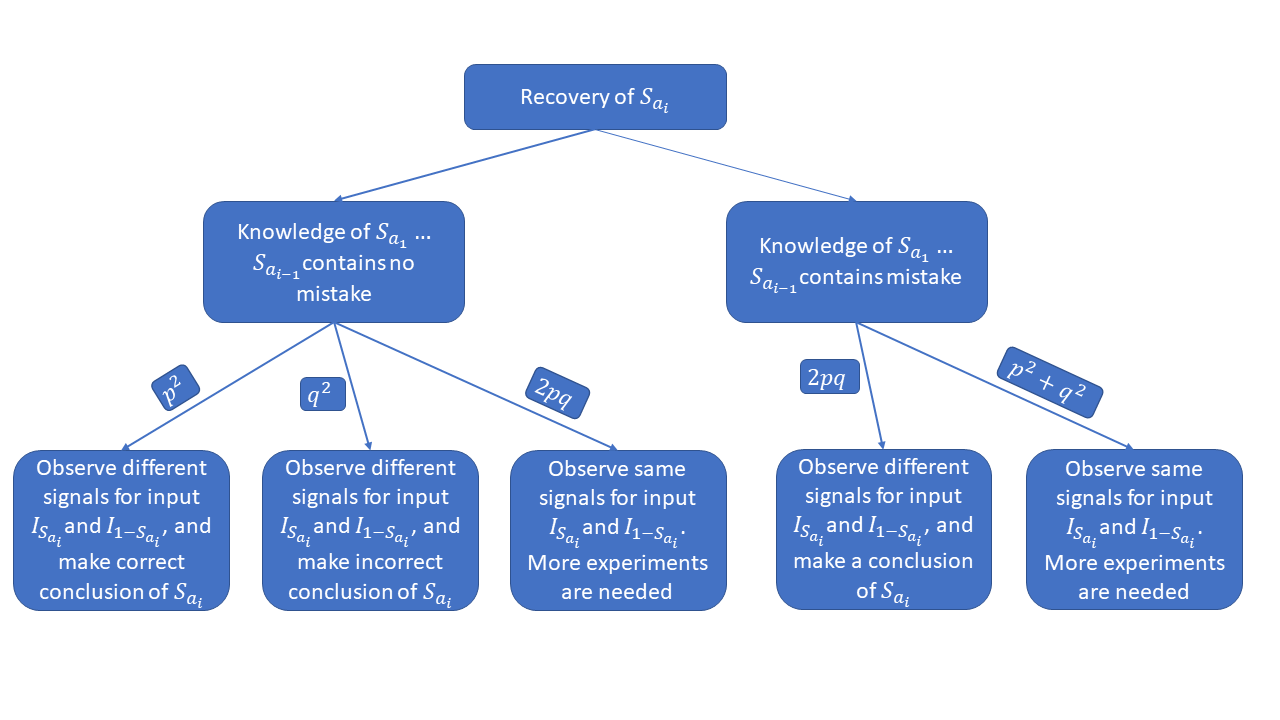
\includegraphics[scale=0.3]{error_route.png}
    \caption{Probability tree diagram for recovery of $s_{a_i}$}
    \label{fig:tree}
\end{figure}

From the attacker's perspective, if he receives different signals for a pair of inputs, he cannot decide whether the signals are correct or not. However, if he receives same signals for a pair of input, he knows that either this experiment failed or he made mistake in previous experiments. To gain more confidence in the current experiment, he would run the experiment for $n$ times, where $n$ should be big enough to distinguish the two cases. We use $x$ to denote the number of experiments that the attacker observes same signals among the $n$ experiments. If mistakes are made in previous experiments, the attacker has $q^2+p^2$ probability to observe same signals in current experiment. He can calculate the range $(r_1, r_2)$ such that the probability of $x$ to be outside the range is negligible:
\begin{equation} \label{eq:1}
    1- \sum_{i=r_1}^{i=r_2} \binom{n}{i} (q^2+p^2)^i(2pq)^{n-i} = \delta
\end{equation}
If no mistake is made in previous experiments, the attacker has $2pq$ probability to observe same signals in current experiment. He can calculate the range $(r_3, r_4)$ such that the probability of $x$ to be outside the range is negligible:
\begin{equation} \label{eq:2}
    1- \sum_{i=r_3}^{i=r_4} \binom{n}{i} (q^2+p^2)^{n-i}(2pq)^{i} = \delta
\end{equation}
Given numerical value of $p$ $q$, the attacker can solve equation \ref{eq:1} and equation \ref{eq:2} together to find an $n$ such that the ranges $(r_1, r_2)$ and $(r_3, r_4)$ don't overlap. After launching the experiment $n$ times, if $x$ fells in the range of $(r_3, r_4)$, he can decide the value of $s_{a_i}$ by taking majority of the $n$ experiments. If $x$ fells in the range of $(r_1, r_2)$, he needs to backtrack since mistakes are made in previous experiments. We summarize the decision tree that the attacker would follow in Figure \ref{fig:backtrack}.

\begin{figure}[h]
    \centering
    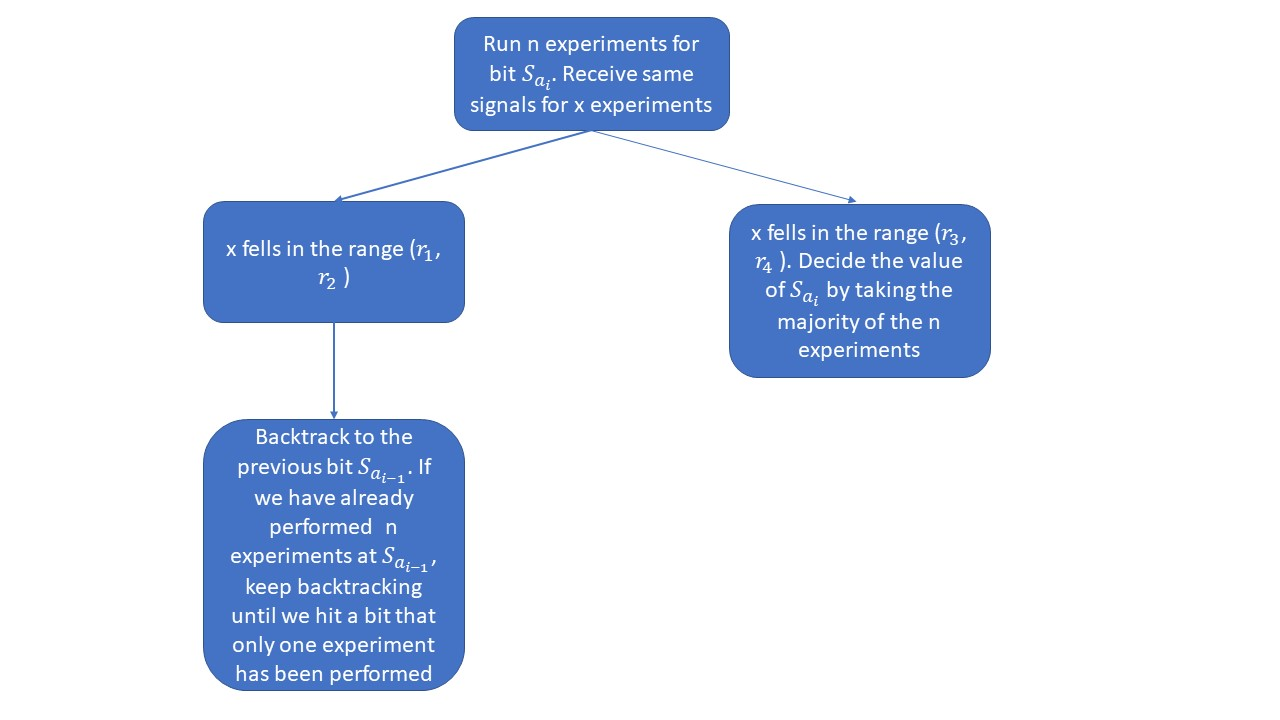
\includegraphics[scale=0.3]{backtrack.jpg}
    \caption{Decision tree for running n experiments}
    \label{fig:backtrack}
\end{figure}

Finally we compute the expected number of experiments should be performed to retrieve the static key $s_a$ of length $k$. 
\begin{lemma}
After a mistake is made, the expected number of bits that the attacker will explore before performing a backtrack is: $\frac{1}{1-2pq}$. 
\end{lemma}
\begin{proof}
Once a mistake is made, the attacker has chance $p^2+q^2$ to observe same signals and $2pq$ to observe different signals. Since he will only explore the following bits if he observes different signals, the chance that he will explore $i$ bits and then realize he made a mistake is: $(2pq)^{i-1}*(p^2+q^2)$. The expected number of bits he will explore is: 
\begin{equation} \label{eq:3}
\begin{split}
    \sum_{i=k}^{i=1} i*(2pq)^{i-1}*(p^2+q^2) & = (p^2+q^2) * (1 + 2(2pq) + 3(2pq)^2 + ... + k(2pq)^{k-1} )\\
                                             & = (p^2+q^2)*(1 + (2pq) + (2pq)^2 + ... + (2pq)^{k-1} ) + \\
                                             &   (p^2+q^2)*( (2pq) + (2pq)^2 + ... + (2pq)^{k-1} ) + \\
                                             &   (p^2+q^2)*( (2pq)^2 + ... + (2pq)^{k-1}) + \\
                                             &   (p^2+q^2) * (2pq)^{k-1}
\end{split}
\end{equation}
Equation \ref{eq:3} can be bounded by:
\begin{equation} \label{eq:4}
\begin{split}
\sum_{i=k}^{i=1} i*(2pq)^{i-1}*(p^2+q^2) & <= (p^2+q^2) * (\frac{1}{1-2pq} + (2pq)*\frac{1}{1-2pq} + \\
                                         &(2pq)^2*\frac{1}{1-2pq} + ... + (2pq)^{k-1}*\frac{1}{1-2pq})\\
                                         & <= (p^2+q^2) * (\frac{1}{1-2pq})^2 = \frac{1}{1-2pq}
\end{split}
\end{equation}
\end{proof}

\begin{lemma}
The expected number of experiments the attacker needs to perform to retrieve the static key $s_a$ of length $k$ is: $k*(p^2+n*(2pq+\frac{q^2}{1-2pq}))$.
\end{lemma}
\begin{proof}
At bit $s_{a_i}$, the attacker has probability $p^2$ to recover the bit with one experiment; probability $2pq$ to recover the bit with $n$ experiments; probability $q^2$ to draw incorrect conclusion of the bit and then backtrack to recover the bit with $\frac{n}{1-2pq}$ experiments. In total he needs to perform $k*(p^2+n*(2pq+\frac{q^2}{1-2pq}))$ experiments.
\end{proof}

\section{Experiment}
\subsection{The Gem5 Simulator}
Due to the lack of the real hardware with a silent zero store performance counter $perf_{zero}$, we use the Gem5 simulator to simulate such a hardware \cite{binkert2011gem5}. Gem5 has been widely used in computer architecture simulations for academic research. It is a combination of two projects: M5, a simulator focuses on full system simulation, and GEMS, a simulator focuses on memory system. Gem5 is dynamically configurable through Python interface and it is extensible through a clean model API. We use Gem5 version 20.
\begin{itemize}
    \item Gem5 supports different ISAs (instruction set architectures) like x86, ARM, Alpha, and RISC-V. 
    \item Gem5 provides system call emulation(SE) and full system emulation(FS). The SE emulates system-level services without modeling devices and the operating system(OS), which means it ignores the timing of many system-level effects including system calls, TLB misses, and device accesses. The FS models the OS and devices and it also executes both user-level and kernel-level instructions. Compare to the SE mode, FS mode is slower in execution but gives a more accurate simulation.
    \item Gem5 supports different CPU models. It supports simple CPU such as AtomicSimpleCPU, a simple one cycle-per-instruction memory model, and TimingSimpleCPU, a simple memory model simulates the timing of memory references. Additionally, It supports CPU models with high-fidelity: a pipelined, in-order CPU model(MinorCPU) and a pipelined, out-of-order CPU model(DerivO3CPU). When using CPU models with high-fidelity, Gem5 runs much slower but gives more realistic results.
    \item Gem5 supports two different cache systems: Ruby and classic caches. Ruby models cache coherence protocols. The classic caches have a single hard-coded hierarchical MOESI coherence protocol. The classic caches can be easily composed to build a hierarchical cache but it does not model the detail of cache coherence well.  
\end{itemize}
\subsection{The Gem5 configuration}
Throughout our experiments, we configure Gem5 as Table \ref{tab:gem5_config}.
\begin{table}[]
\begin{tabular}{ll}
Gem5 mode                           & Full system                            \\
CPU model                           & X86 Out-of-order CPU                   \\
CPU clock                           & 2GHz                                   \\
CPU fetch width                     & 8 instructions per cycle               \\
Number of CPU                       & 1                                      \\
Number of hyperthreads in a CPU     & 1                                      \\
OS                                  & Gentoo Linux                           \\
Kernel                              & Linux 5.7                              \\
L1 data cache                       & 16KB, 4 way (private)                  \\
L1 instruction cache                & 16KB, 4 way (private)                  \\
L1 data latency                     & 2 cycles                               \\
L1 response latency                 & 2 cycles                               \\
L2 cache size                       & 1MB, 8 way  (shared, and exclusive)    \\
L2 data latency                     & 20 cycles                              \\
L2 response latency                 & 20 cycles                              \\
Cacheline size                      & 64 bits                                \\
Physical memory size                & 4GB                                    \\
Dynamic Random-Access Memory module & DDR3\_1600\_8x8 (12.8 GBps throughput)
\end{tabular}
\caption{The Gem5 configuration for full system mode}
\label{tab:gem5_config}
\end{table}

\subsection{The Gem5 silent zero store performance counter and silent zero store} 
We implement two versions of hardware silent zero store performance counter in Gem5: a full cacheline version $perf_{zero}$, with which we record the number of redundant zeros overwriting zeros of a full cacheline(64 bits), and a half cacheline version $perf_{halfzero}$, with which we record the number of redundant zeros overwriting zeros of a half cacheline(32 bits), which is either the top half of a cacheline of the bottom half of a cacheline.

\textbf{Full cacheline silent zero store performance counter: }Upon allocation of a cache line, we record the cacheline address (cache tag and cache index) if it contains only 0. Upon eviction of the cacheline, if it is dirty and still contains only 0, we increment $perf_{zero}$ and remove the cacheline from our record.

\textbf{Half cacheline silent zero store performance counter: }Upon allocation of a cacheline, we record the top half of it if the addresses at offset between 0 and 31 contain only 0, and we record the bottom half of it if the addresses at offset between 32 and 63 contain only 0. We mark both the top and bottom half as clean upon allocation. During future writes to the cacheline, we mark the top half of it as dirty if any write modifies the addresses at offset between 0 and 31, and bottom half of it as dirty if any write modifies the addresses at offset between 32 and 63. Upon eviction of the cacheline, if the top half of it is dirty and still contains only 0, we increment $perf_{halfzero}$. We do the same check to the bottom half of the cacheline. We remove the top and bottom half of the cacheline from our record. 

\textbf{The Gem5 silent zero store}
We implement a full cacheline version silent zero store for both L1 and L2 cache in Gem5. Specifically, for any writeback that is a silent zero store, we treat it as a clean eviction.

\subsection{The Gem5 shadow silent zero store performance counter} 
We aim to minimize the number of iterations we need to execute a binary to carry out an attack. For a given protocol, we only interest in the change of $perf_{zero}$ of a specific function (e.g. the key decapsulation function in the SIKE protocol). We attempt to get rid of the influence of other operations like loading the private and public keys. We borrow the idea from the King et al \cite{king2008designing}, and implement a shadow silent zero store performance counter. Our shadow silent zero store performance counter lies in-between pure hard-ware and pure software. 

Before the execution of a function of our interests, we allocate a buffer of the same size as a packet (64bits) in Gem5, and the buffer contains a backdoor byte sequence $\{0xb4,0xaf,0x98,0x1a,0xfc,0x96,0x08,0x06\}$. Once the CPU inspects a packet containing this sequence, it activates $perf_{zero}$. After the execution of the same function, we allocate another buffer containing another backdoor byte sequence $\{0xfc,0x96,0x08,0x06,0xb4,0xaf,0x98,0x1a\}$ to deactivate $perf_{zero}$. Our backdoor byte sequences are long enough such that the chance of a normal packet happens to activate or deactivate $perf_{zero}$ is negligible. 


\subsection{Target Implementations}
We use silent zero store performance counter to attack the following implementation: \textbf{RSA(4096)} decryption in the 3.0.0-alpha7-dev version of OpenSSL with precomputed CRT and RSA blinding turned off. The secret key size is 4096 bits long \cite{openssl}. \textbf{ECDH(521)} decryption in the 1.0.2u version of OpenSSL. Our curve is $secp521r1$, which contains a point with x coordinate equals to 0. The secret key size is 521 bits long. We choose 1.0.2u version because it doesn't blind the projective (homogeneous) coordinates. OpenSSL 1.0.2u uses the Montgomery Ladder Algorithm \ref{tab:algML} for scalar multiplication of elliptic curve points \cite{openssl}. \textbf{ECDH(256)} decryption in the 1.15.6 version of Golang. Our curve is $secp256r1$ which contains a point with x coordinate equals to 0. The secret key size is 256 bits long. Golang 1.15.6 doesn't blind the projective (homogeneous) coordinates. It uses the Fixed window Algorithm \ref{tab:algFW} with window size $w=5$ for scalar multiplication of elliptic curve points \cite{donovan2015go}. \textbf{SIKE} key decapsulation in the Cloudflare Interoperable Reusable Cryptographic Library (Circl) \cite{circl}. The secret key size is 378 bits long. The prime field of the elliptic curve is 751 bits long. Circl implements the three point ladder Algorithm \ref{tab:Ladder3pt} for computing $\phi_B(P_A) + [sk_A]\phi_B(Q_A)$ and there is no input verification for the key decapsulation function. 

We add activation backdoor byte sequence before the decryption/decapsulation function, deactivation backdoor byte sequence after the decryption/decapsulation function. We add memory barriers to ensure the order of the functions and backdoor sequences. For RSA(4096), ECDH(521), and SIKE, we use the $perf_{zero}$ to count the change of the silent zero store number before and after the function, since the prime numbers and prime fields used by them are big enough to cover a full cacheline. For ECDH(256), we use the $perf_{halfzero}$ count the change of the silent zero store number before and after the function, because the prime field used by ECDH(256) is only big enough to cover half of the cacheline. We target the ECDH(256) case of Golang because Golang doesn't have a constant time implementation of the ECDH(521). We argue that the $perf_{halfzero}$ of the ECDH(256) case can be extended to $perf_{zero}$ of ECDH(521). 

\subsection{Experiment Result}


\section{Side Channel Attack}
In a real server, accessing the performance counters usually requires the root privilege, so it is unlikely that the attacker can get access to the $perf_{zero}$ and $perf_{halfzero}$ before and after the execution of a function. To illustrate that the silent zero store can be used as a side channel, we perform a proof-of-concept side channel attack.

\subsection{The Gem5 configuration}
Throughout our experiments, we configure Gem5 as Table \ref{tab:gem5_config_se}. We use the system emulation mode to launch this attack because the full system mode doesn't support multiple X86 out-of-order CPUs with classic memory\cite{gem5fail}. We use WideIO\_200\_1x128 as our DRAM because it has smaller throughput compare to DDR3\_1600\_8x8 so it is easier to saturate the DRAM bandwidth. 
\begin{table}[]
\begin{tabular}{ll}
Gem5 mode                           & System emulation                       \\
CPU model                           & X86 Out-of-order CPU                   \\
CPU fetch width                     & 8 instructions per cycle               \\
Number of CPU                       & multi-cores                            \\
CPU clock                           & 2GHz                                   \\
Number of hyperthreads in a CPU     & 1                                      \\
L1 data cache                       & 16KB, 4 way (private)                  \\
L1 instruction cache                & 16KB, 4 way (private)                  \\
L1 data latency                     & 2 cycles                               \\
L1 response latency                 & 2 cycles                               \\
L2 cache size                       & 1MB, 8 way  (shared, and exclusive)    \\
L2 data latency                     & 20 cycles                              \\
L2 response latency                 & 20 cycles                              \\
Cacheline size                      & 64 bits                                \\
Physical memory size                & 4GB                                    \\
Dynamic Random-Access Memory module & WideIO\_200\_1x128 (3.125 GBps throughput)
\end{tabular}
\caption{The Gem5 configuration for system emulation mode}
\label{tab:gem5_config_se}
\end{table}


\subsection{The attack setup and result}
Our proof-of-concept side channel attack works as following: Setting up a multi-cores system ($c$ denotes the number of cores) with silent zero store enabled, we launch one process per core. The workload of each process is 1. allocate a buffer of size $10^8$, and 2. overwrite the whole buffer with $0$ or $1$ twice. Define $Exp_A$ as the experiment that, one of the process writes $0$ and the other processes write $1$. For one of the writing $1$ processes we measure the time $time(Exp_A)$ that it takes to finish the workload. Define $Exp_B$ as the experiment that, every process writes $1$. For one of processes we measure the time $time(Exp_B)$ that it takes to finish the workload. The buffer size ($10^8$) is much larger than the L2 cache size, so during overwritings, many cachelines will be evicted from the cache. 

In $Exp_A$, one of the process only writes $0$, almost all of its writebacks will be dropped. There are $c$ processes read and $c-1$ processes write. In $Exp_B$, every process writes $1$. There are $c$ processes read and $c$ processes write. Let $Read_{percentage}$ denote the data bus utilization in percentage for reads; $Write_{percentage}$ denote the data bus utilization in percentage for writes; $Total_{percentage}$ denote the data bus utilization in percentage for reads plus writes. The DRAM WideIO\_200\_1x128 has one command and address bus which takes care of both reading and writing requests. Therefore, there should be less pressure on DRAM bandwidth in $Exp_A$ compare to that of $Exp_B$. $time(Exp_A)$ should be smaller than $time(Exp_B)$ for the side channel attack to succeed. 

We launch $Exp_A$ and $Exp_B$ for the number of cores $c$ equals to $2$, $3$, $4$, $6$, $7$, $12$. We plot ($time(Exp_A)$, $time(Exp_B)$) versus $c$ in Figure \ref{fig:timeAB} and ($Read_{percentage}$, $Write_{percentage}$, $Total_{percentage}$) versus $c$ for $Exp_A$ and $Exp_B$ in Figure \ref{fig:databus}.

In Figure \ref{fig:databus}, the data bus saturates at $c=6$. As we expected, for $Exp_B$, data bus utilization in percentage for reads and writes are the same; for $Exp_A$, $\frac{Read_{percentage}}{Write_{percentage}} = \frac{c}{c-1}$, which means that the DRAM distributes its bandwidth to reads and writes according to the ratio of the number of reading requests and writing requests.  

In Figure \ref{fig:timeAB} (a), regardless the value of $c$, $time(Exp_A)$ is always smaller than $time(Exp_B)$. We further investigate the relationship between ($time(Exp_A)$, $time(Exp_B)$) and $c$. As we can see in Figure \ref{fig:timeAB} (b), once the DRAM bandwidth is saturated (after $c=6$), $\frac{time(Exp_A)}{time(Exp_B)} = \frac{2c-1}{c}$, which means that in $Exp_A$, DRAM bandwidth is evenly distributed among $c$ reads and $c-1$ writes, and in $Exp_B$, DRAM bandwidth is evenly distributed among $c$ reads and $c$ writes. Therefore, regardless of whether the bandwidth is saturated or not, we are able to observe a performance speedup in $Exp_A$ compare to that of $Exp_B$. These pair of experiments proves that the silent zero store can be used as a side channel to mount attacks.


\begin{figure}%
    \centering
    \subfloat[\centering]{{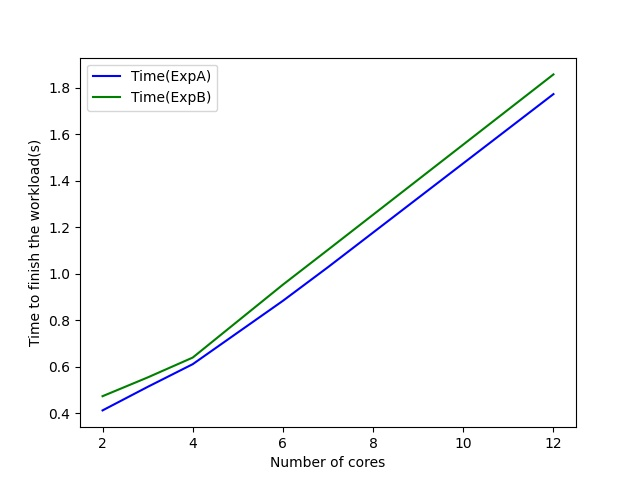
\includegraphics[scale=0.35]{timeAB.jpg} }}%
    \qquad
    \subfloat[\centering]{{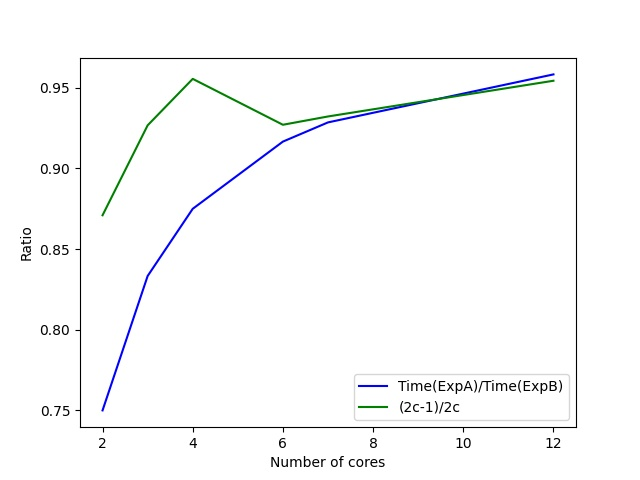
\includegraphics[scale=0.35]{ratio.jpg} }}%
    \caption{($time(Exp_A)$, $time(Exp_B)$) versus number of cores}%
    \label{fig:timeAB}%
\end{figure}

\begin{figure}%
    \centering
    \subfloat[\centering $Exp_A$]{{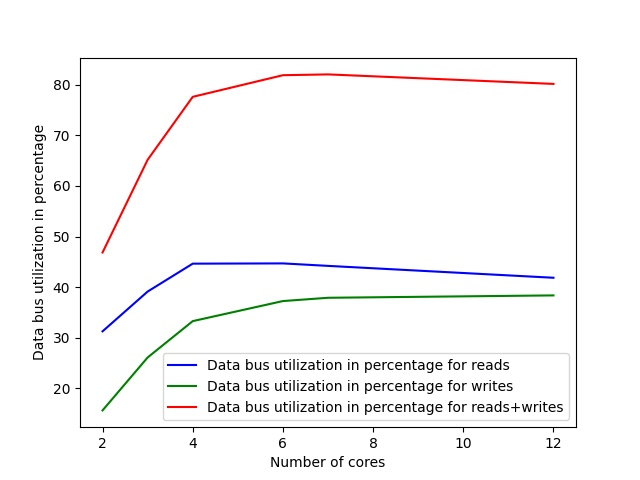
\includegraphics[scale=0.35]{data_util_1_0.jpg} }}%
    \qquad
    \subfloat[\centering $Exp_B$]{{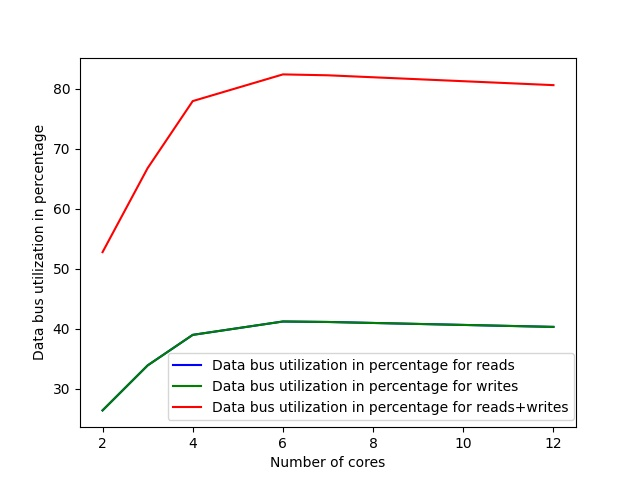
\includegraphics[scale=0.35]{data_util_1_1.jpg} }}%
    \caption{Data bus utilization versus number of cores for $Exp_A$ and $Exp_B$}%
    \label{fig:databus}%
\end{figure}
\section{Defenses}

\bibliographystyle{unsrt}
\bibliography{ref}
\end{document}
